\documentclass{article}

\usepackage[T1]{fontenc} % Umożliwia korzystanie z fontów o kodowaniu T1, które obsługują znaki specjalne używane w językach europejskich.
\usepackage[polish]{babel} % Dostosowuje formatowanie dokumentu do zasad języka polskiego (np. łamanie wierszy, tytuły sekcji).
\usepackage[utf8]{inputenc} % Umożliwia korzystanie z kodowania UTF-8, które obsługuje znaki specjalne i diakrytyczne.
\usepackage{graphicx} % Umożliwia wstawianie obrazów do dokumentu.
\usepackage{subcaption} % Umożliwia tworzenie podpisów dla podobrazów.
\usepackage[margin=2cm]{geometry} % Umożliwia dostosowanie marginesów dokumentu.
\usepackage{listings} % Umożliwia wstawianie kodu źródłowego do dokumentu z odpowiednim formatowaniem.
\usepackage{color} % Umożliwia korzystanie z kolorów w dokumencie.
\usepackage{amsmath} % Rozszerza możliwości formatowania równań matematycznych.
\usepackage{xcolor} % Umożliwia tworzenie kolorowych ram dookoła tekstu.
\usepackage{systeme} % Umożliwia tworzenie systemów równań.
\usepackage{indentfirst} % Powoduje, że pierwszy akapit po tytule sekcji jest wcięty.
\usepackage{dsfont} % Umożliwia korzystanie z dodatkowych fontów, np. dla oznaczeń zbiorów liczbowych.
\usepackage{etoolbox} % Pozwala modyfikować pakiety UŻYWAĆ OSTROŻNIE
\usepackage{blindtext} % Pozwala automatycznie pisać blok lorem ipsum
\usepackage{fancyhdr} % Pozwala na stopki u góry i na dole strony
\usepackage{hyperref} % Umożliwia używanie hyperlinków
\usepackage[justification=centering]{caption}
\hypersetup{
  colorlinks = true,
  linkcolor = black,
  urlcolor = blue,
  pdftitle = {Sprawozdanie z Laboratorium 4} 
}
\patchcmd{\section}{\thispagestyle{plain}}{\thispagestyle{fancy}}{}{}

\definecolor{red}{RGB}{245, 63, 60}
\definecolor{blue}{RGB}{59, 69, 245}
\definecolor{green}{RGB}{72, 225, 17}
\definecolor{yellow}{RGB}{245, 207, 59}

\begin{document}
  \pagestyle{fancy} % pozwala korzystać z pakietu fancyhdr
  \fancyhf{} % clear existing header/footer entries
  \fancyfoot[C]{\thepage}
  \renewcommand{\headrulewidth}{0pt} % Usuń linię na górze strony
  \renewcommand{\footrulewidth}{0.4pt} % Dodaj linię na dole strony  
  \addtolength{\footskip}{0cm} % Zmienia pozycję linii w stopce

  \title{Elektronika Cyfrowa \\ {\large Sprawozdanie z Laboratorium 4}}
  \date{24.04.2024}
  \author{Tomasz Dziób\\{\small Grupa 15}}
  \maketitle

  % Ustawienie Spisu treści do paragrafów 
  \setcounter{tocdepth}{4} % Uwzględnij do typu \paragraph in Spisie treści
  \setcounter{secnumdepth}{4} % Numerowanie do typu \paragraph
  \small \tableofcontents
  \pagebreak

  \section{Wstęp teoretyczny}
  Poniższe sprawozdanie dotyczy dotyczy czwartych zajęć których głównym celem było zapoznanie się z podstawami elektroniki cyfrowej czli bramkami logicznymi. 
    \subsection{Algebra Boole'a}
    Algebra Boole'a jest strukturą matematyczną gdzie dany jest:
    \begin{itemize}
      \item zbiór dwuelementowy
      \item działania alternatywy (sumy)
      \item koniunkcji (iloczynu)
      \item negacji (dopełnienia)
    \end{itemize}
    Dla uproszczenia zapisu koniunkcję $p \land q$ zapisujemy jako $p \cdot q$ lub $pq$, a negację jako $\lnot p$ lub $\overline{p}$. Poniżej prezentuje jedne z ważniejszych praw alegbry Boole'a:

    \begin{table}[h]
      \centering
      \begin{tabular}{|c|c|c|}
      \hline
      \textbf{Prawo} & \textbf{Iloczyn} & \textbf{Alternatywa}\\
      \hline
      \textbf{Prawo rozdzielności}  & \footnotesize $A(B + C) = AB + AC$ & \footnotesize $A + (BC) = (A + B)(A + C)$\\
      \hline
      \textbf{Prawo tożsamości} & \footnotesize $ 1\cdot A = A$ & \footnotesize $ 0 + A = A$\\
      \hline
      \textbf{Prawo odwrotności} & \footnotesize $ A\cdot \overline{A} = 0$ & \footnotesize $ A + \overline{A} = 1$\\
      \hline
      \textbf{---} & \footnotesize $ 0 \cdot A = 0$ & \footnotesize $ 1 + A = 1$\\
      \hline
      \textbf{---} & \footnotesize $ A\cdot A = A$ & \footnotesize $ A + A = A$\\
      \hline
      \textbf{Prawa De Morgana} & \footnotesize $ \overline{(A \cdot B)} = \overline{A} + \overline{B}$ & \footnotesize $ \overline{(A + B)} = \overline{A} \cdot \overline{B}$\\
      \hline
      \end{tabular}
      \caption{Podstawowe prawa działania algebry Boole'a}
      \end{table}

    \subsection{Układy cyfrowe}
      Układ cyfrowy, znany również jako układ logiczny, to układ przeprowadzający działania na danych wejściowych i wypuszczający je na kanały wyjściowe. Układy cyfrowe są budowane w oparciu o bramki logiczne, które realizują elementarne operacje logiczne.
      Układy cyfrowe są zaprojektowane do realizacji takich zadań jak przetwarzanie informacji (w tym obliczenia) oraz sterowanie urządzeniami i innymi systemami lub obiektami.

      Układy cyfowe możemy podzielić na układy kombinacyjne oraz sekwencyjne.
      \subsubsection{Układy kombinacyjne}
        W takich układach stan wyjść jest jednoznacznie określony przez stan wejść układu.
        W prostszych słowach, są to układy \textit{"bez pamięci"}, w których sygnały wyjściowe są zawsze takie same dla określonych sygnałów wejściowych.

      
      \subsubsection{Układy sekwencyjne}
        W układach sekwencyjnych stan wyjść zależy od stanu wejść oraz od poprzednich stanów układu.
        Czyli można powiedzieć że \textit{"pamiętają"} one, stany wcześniejsze i wpływa to na następne wyniki.

        W tym przypadku można wyróżnić jeszcze jeden podział: na układy sekwencyjne asynchroniczne i synchroniczne.
        \paragraph{Asynchroniczne}
          \mbox{}\newline
          W układach asynchronicznych zmiana sygnałów wejściowych natychmiast powoduje zmianę wyjść. W związku z tym układy te są szybkie, ale jednocześnie podatne na zjawisko hazardu i wyścigu, czyli gdy co najmniej dwa sygnały wejściowe zmieniają swój stan w jednej chwili.

        \paragraph{Synchroniczne}
          \mbox{}\newline
          W układach synchronicznych zmiana stanu wewnętrznego następuje wyłącznie w określonych chwilach, które wyznacza sygnał zegarowy. Każdy układ synchroniczny ma wejście zegarowe oznaczane zwyczajowo symbolami C, CLK lub CLOCK.
    
    \subsection{Mapy Karnaugha}
    Mapy Karnaugha to metoda upraszczania wyrażeń logicznych algebry Boole'a. Odwzorowuje ona sygnały wejściowe układu w sygnały wyjściowe. Oznacza to, że część zmiennych binarnych przypisana jest wierszom, a część kolumnom. Indeksy i kolumny numerowane są przy pomocy kodu Graya.
    Grupowanie osobno jedynek lub zer pozwala uzyskać różne schematy budowy układu. Po zapisaniu równania, można je uprościć zasadami algebry Boole'a aby uzyskać najoptymalniejszą wersję układu.

    Mapy Karnaugh są szeroko stosowane w kombinacyjnych układach logicznych w celu uproszczenia i zapobiegania potencjalnym warunkom wyścigu. Dzięki zastosowaniu kodu Graya możliwe jest znalezienie w wizualny sposób pól sąsiednich logicznie, czyli różniących się wartością dokładnie jednej zmiennej.
      \begin{figure}[!ht]
        \centering
        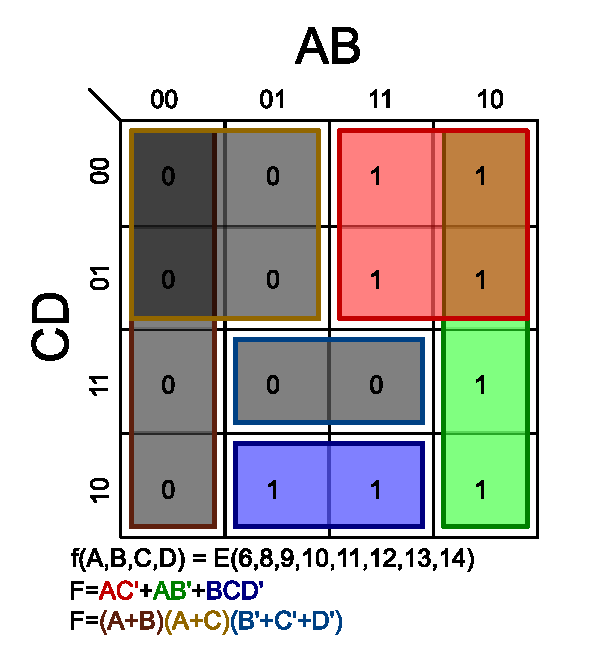
\includegraphics[scale=0.55]{grafiki/K-map.eps}
        \caption{Przykładowa mapa Karnaugha,
        \\Źródło: \href{https://en.m.wikipedia.org/wiki/File:K-map_6,8,9,10,11,12,13,14.svg}{Wikipedia}}
      \end{figure}
    
    \subsection{Bramki logiczne}
      Są to element konstrukcyjne mechanizmów realizujących funkcję logiczną, której argumenty (zmienne logiczne) oraz sama funkcja mogą przybierać jedną z dwóch wartości, np. 0 lub 1 (jak w algebrze Boole'a).

      Bramki te realizują głównie operacje logiczne takie jak negacja iloczyn oraz suma, jednak istnieją też ich zanegowane wersje jak i operacja wyłącznej sumy logicznej.

      \begin{figure}[!ht]
        \centering
        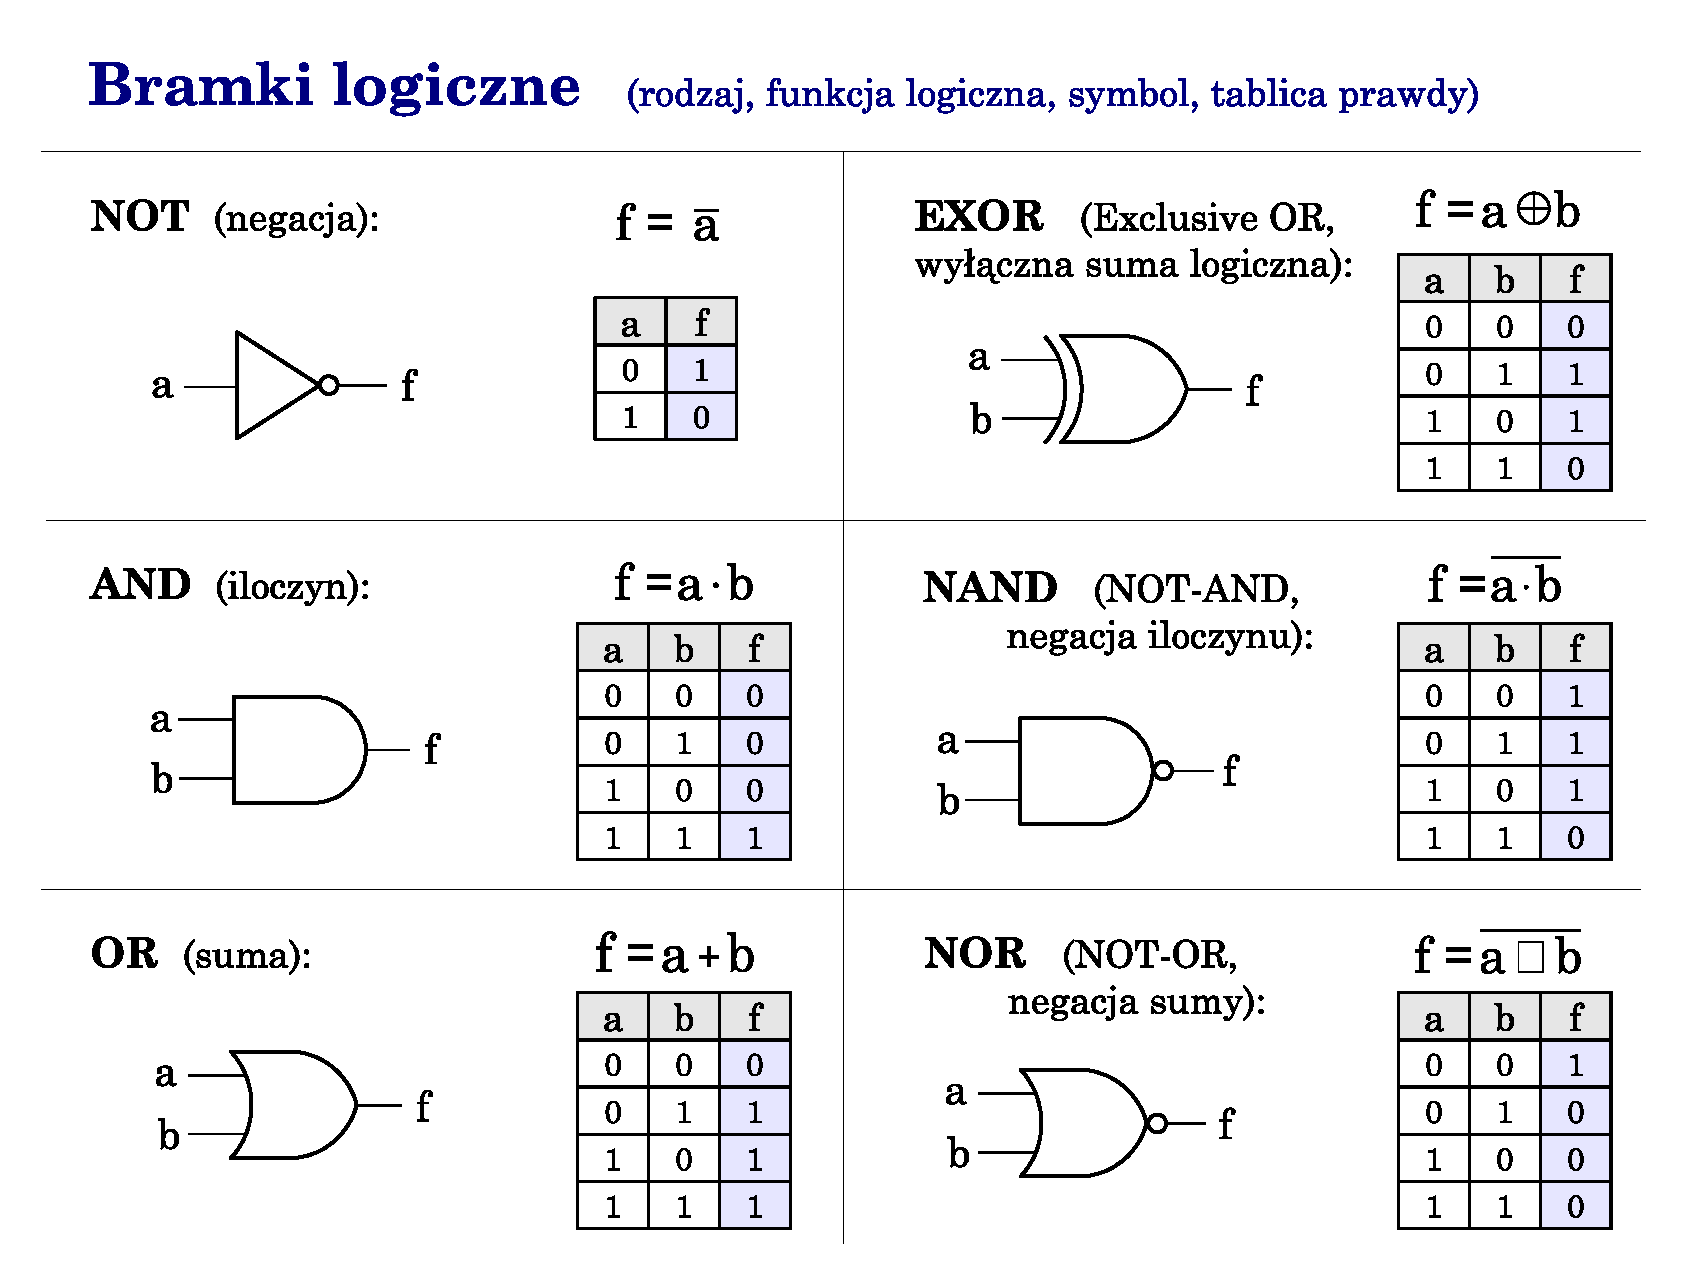
\includegraphics[scale=0.35]{grafiki/Bramki_logiczne.eps}
        \caption{Rodzaje bramek logicznych, ich symbole oraz tablice prawdy,
        \\Źródło: \href{https://spe.if.uj.edu.pl/literatura}{Strona wykładów}}
        \label{fig2:brameczki}
      \end{figure}

      Tablica prawdy --- to lista wszystkich możliwych stanów osiąganych przez bramkę dla wszyskich istniejących kombinacji danych wejściowych. Pokazuje ona w prosty i szybki sposób działanie bramki.

      \subsubsection{Podstawowe operacje zbudowane z bramek}
        Bramki \textbf{NAND} (negacja koniunkcji) oraz \textbf{NOR} (negacja sumy logicznej) nazywa się \underline{funkcjonalnie pełnymi} lub \underline{zupełnymi} ponieważ z każdej z nich można zbudować \textcolor{green}{układ realizujący dowolną funkcję logiczną}.
        \\\\
        Oto przykłady operacji logicznych zrealizowanych przy pomocy bramek NAND oraz NOR:

        \begin{figure}[!ht]
          \centering
          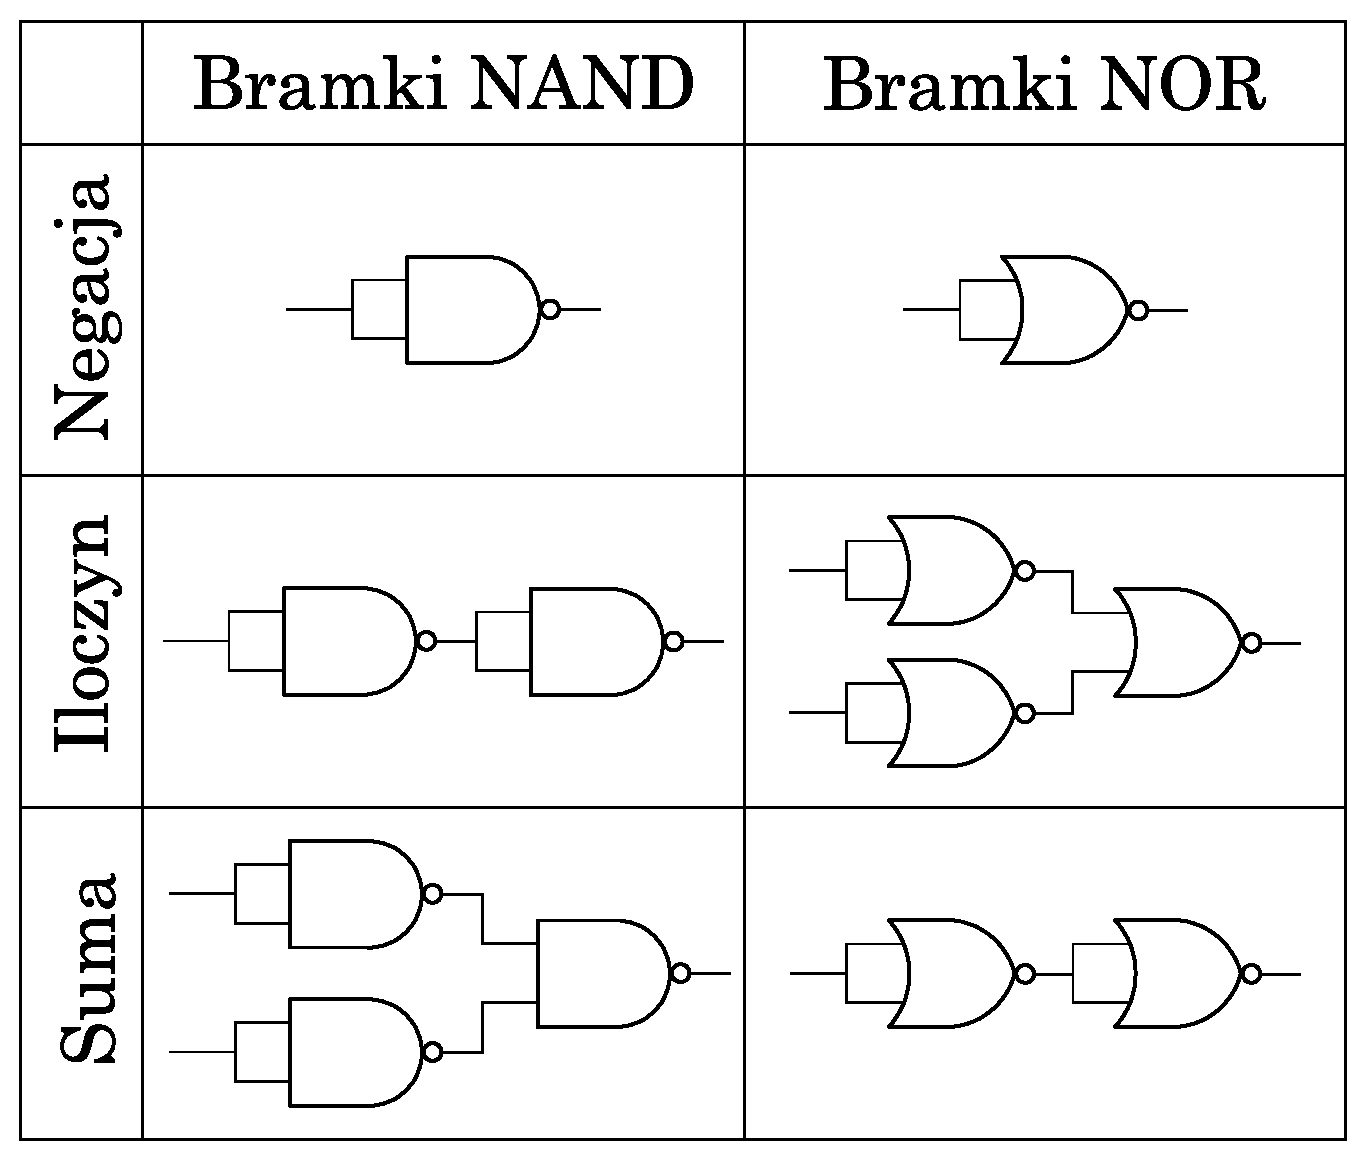
\includegraphics[scale=0.3]{grafiki/Operacje.eps}
          \caption{Schematy operacji logicznych zrealizowanych przy pomocy bramek NAND oraz NOR,
          \\Źródło: Opracowanie własne}
          \label{fig1:Operacje}
        \end{figure}
      
      \subsubsection{Układy TTL}
        Ze względu na stosowane technologie, bramki logiczne tworzą tzw. rodziny (np. TTL ECL, CMOS). Jedną z najbardziej rozpowszechnionych jest rodzina bramek TTL (Transistor - Transistor Logic). Ten typ bramek był również wykorzystywany na podczas zajęć.

        \paragraph{Charakterystyka układów TTL}
        \begin{itemize}
          \item Układy pracują w logice dodatniej
          \item Logicznemu zeru (L --- stan niski) odpowiada napięcie z przedziału: \\
          0 ---  0.8 V (sygnały wejściowe) \\
          0 --- 0.4 V (sygnały wyjściowe) \\
          \item Logicznej jedynce (H --- stan wysoki) odpowiada napięcie z zakresu: \\
         2.0 -- 5 V (sygnały wejściowe) \\
         2.7 --- 5 V (sygnały wyjściowe) \\
          \item Wejście bramki niepodłączone do niczego
          znajduje się w stanie logicznym 1
          \item Układy zasila się napięciem +5 V
        \end{itemize}

    \subsection{Asynchroniczny przerzutnik RS}
      \textit{Przerzutnik typu RS} to najprostszy rodzaj przerzutnika asynchronicznego. Można go zbudować zarówno z dwóch bramek logicznych \textit{NOR} lub dwóch bramek logicznych \textit{NAND}. Przerzutnik RS ma dwa wejścia i dwa wyjścia: \\ 
      \pagebreak
      Wejścia: \\
      \textbf{S} (Set) --- wejście ustawiające \\
      \textbf{R} (Reset) --- wejście zerujące \\

      Wyjścia: \\
      \textbf{Q} --- wyjście zwykłe (główne) \\
      $\mathbf{\overline{Q}}$ --- wyjście zanegowane (komplementarne) \\

      \begin{figure}[!ht]
        \begin{minipage}{.5\textwidth}
            \centering
            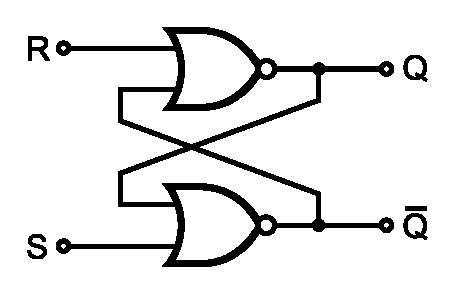
\includegraphics[scale=0.87]{grafiki/RS_NOR.eps}
            \caption{Schemat realizacji przerzutnika RS z bramek NOR,
            \\Źródło: \href{https://pl.wikipedia.org/wiki/Plik:RS_Flip-flop_(NOR).svg}{Wikipedia}}
        \end{minipage}
        \begin{minipage}{.5\textwidth}
            \centering
            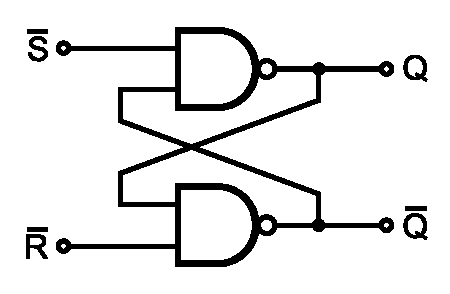
\includegraphics[scale=0.87]{grafiki/SR_NAND.eps} 
            \caption{Schemat realizacji przerzutnika SR z bramek NAND,
            \\Źródło: \href{https://pl.wikipedia.org/wiki/Plik:SR_Flip-flop_Diagram.svg}{Wikipedia}}
        \end{minipage}
      \end{figure}

      Przerzutnik RS działa na zasadzie sprzężenia zwrotnego, gdzie wyjścia są podłączone do wejść. Dzięki temu przerzutnik jest w stanie utrzymać ostatni stan wyjść, nawet po przejściu stanów logicznych na wejściach w stan neutralny (nic nie jest podpięte na wejścia).
      Stan, w którym oba wejścia są w stanie wysokim, jest \underline{stanem zabronionym}. Jest on niezgodny z 
      definicją stanów wyjściowych przerzutnika.

      \begin{table}[h]
        \centering
        \begin{tabular}{|c|c|c|c|}
        \hline
        \footnotesize \textbf{S} & \footnotesize \textbf{R} & \footnotesize $\mathbf{Q_n}$ & \footnotesize $\mathbf{\overline{Q_n}}$ \\
        \hline
        0 & 0 & stan pamiętania & stan pamiętania \\
        \hline
        0 & 1 & 0 & 1 \\
        \hline
        1 & 0 & 1 & 0 \\
        \hline
        1 & 1 & stan zabroniony & stan zabroniony \\
        \hline
        \end{tabular}
        \caption{Tablica prawdy dla przerzutnika RS zbudowanego na bramkach NOR}
      \end{table}
        

  \section{Ćwiczenia}
    \subsection{Ćwiczenie 4.1}
    Pierwsze zadanie polegało na zapoznaniu się z płytką UC-2 do badania układów scalonych TTL. Zostały przeprowadzone wnikliwe badania wszystkich oferowanych funkcji przez płytkę, w celu upewienia się, że funkcjonuje ona poprawnie.

    \begin{figure}[!ht]
      \centering
      \includegraphics[scale=0.05]{grafiki/sama_plytka.png}
      \caption{Płytka UC-2 do badania układów scalonych TTL używana podczas zajęć,
      \\Źródło: Opracowanie własne}
    \end{figure}

    W pierwszej kolejności zostały sprawdzone piny zasilające $5V$, znajdujące się przy mocowaniach do układów TTL. Oba wskazały równo odczyt 5V podczas pomiarów miernikiem.

    Następnie dokonany został pomiar dotyczący działania diod wskaźnika. Żadna z nich nie wskazała nieprawidłowego działania.

    \subsubsection{Sprawdzenie poprawności działania impulsatorów}
      Do wykonania powyższych pomiarów został wykorzystany oscyloskop. Oba impulsatory zostały wpięte do oscyloskopu w celu wizualizacji zmiany napięcia w czasie.
      
      \begin{figure}[!ht]
        \centering
        \includegraphics[scale=0.15]{grafiki/impulsatory.png}
        \caption{Realizacja podpięcia impulsatorów do oscyloskopu,
        \\Źródło: Opracowanie własne}
      \end{figure}
       Górny impulsator został wpięty na kanał pierwszy a dolny na kanał drugi.

      \begin{figure}[!ht]
        \begin{minipage}{.5\textwidth}
            \centering
            \includegraphics[scale=0.35]{grafiki/gora_Q.png}
            \caption{Zmiana w czasie wyjścia $Q$ górnego impulsatora z widocznym momentem wciśnięcia przycisku,
            \\Źródło: Opracowanie własne}
        \end{minipage}
        \begin{minipage}{.5\textwidth}
            \centering
            \includegraphics[scale=0.35]{grafiki/gora_NQ.png} 
            \caption{Zmiana w czasie wyjścia $\overline{Q}$ górnego impulsatora z widocznym momentem wciśnięcia przycisku,
            \\Źródło: Opracowanie własne}
        \end{minipage}
      \end{figure}

      \begin{figure}[!ht]
        \begin{minipage}{.5\textwidth}
            \centering
            \includegraphics[scale=0.35]{grafiki/dol_Q.png}
            \caption{Zmiana w czasie wyjścia $Q$ dolnego impulsatora z widocznym momentem wciśnięcia przycisku,
            \\Źródło: Opracowanie własne}
        \end{minipage}
        \begin{minipage}{.5\textwidth}
            \centering
            \includegraphics[scale=0.35]{grafiki/dol_NQ.png} 
            \caption{Zmiana w czasie wyjścia $\overline{Q}$ dolnego impulsatora z widocznym momentem wciśnięcia przycisku,
            \\Źródło: Opracowanie własne}
        \end{minipage}
      \end{figure}
      \pagebreak
    \subsubsection{Sprawdzenie poprawności działania diod próbnika}
      Sprawdzenie to miało na celu uniknięciu błędów na późniejszym etapie ćwiczeń, gdzie próbnik diod led był często używany. Test polegał na sprawdzeniu wszystkich możliwych kombinacji które dało się uzyskać z dwoma impulsatorami.
      
      \begin{figure}[!ht]
        \centering
        \includegraphics[scale=0.15]{grafiki/imp_gora_test.png}
        \caption{Seria zdjęć ukazująca działanie próbnika diod dla podłącznego górnego impulsatora,
        \\Źródło: Opracowanie własne}
      \end{figure}

      Na obu seriach zdjęć widzimy sprawdzenia dla sytuacji gdy przycisk nie był wcisnięty oraz gdy był. Sprawdzenie zostało przeprowadzone dla obu wejść $Q$ oraz $\overline{Q}$.
    
      \begin{figure}[!ht]
        \centering
        \includegraphics[scale=0.15]{grafiki/imp_dol_test.png}
        \caption{Seria zdjęć ukazująca działanie próbnika diod dla podłącznego dolnego impulsatora,
        \\Źródło: Opracowanie własne}
      \end{figure}

      Przedstawiając to w formie tabelki:

      \begin{table}[h]
        \centering
        \begin{tabular}{|c|c|c|c|c|}
        \hline
        \footnotesize \textbf{Impulsator}  & \footnotesize $\mathbf{Q}$ & \footnotesize $\mathbf{\overline{Q}}$ & \footnotesize $\mathbf{Q}$ oraz wciśnięty przycisk& \footnotesize $\mathbf{\overline{Q}}$ oraz wciśnięty przycisk \\
        \hline
        \textbf{Górny} & 0 & 1 & 1 & 0\\
        \hline
        \textbf{Dolny} & 0 & 1 & 1 & 0\\
        \hline
        \end{tabular}
        \caption{Prezentacja działania diod próbnika dla dwóch różnych impulsatorów}
      \end{table}

    \subsection{Ćwiczenie 4.2}
      Zadanie drugie dotyczyło badania tablic logicznych bramek NAND, NOR oraz EXOR. Do tego zadania zostały użyte układy scalone odpowiednio o numerach 7400, 7402 oraz 7486.
      \subsubsection{NAND(7400)}
        W celu zbadania wejść oraz wyjść wpierw został sporządzony schemat działania układu. Wykorzystana została do tego dokumentacja układu dostępna w Internecie. Przedstawiony poniżej rysunek został zmodyfikowany tak, jak opisane są wejścia na płytce UC-2 w celu uproszczenia opisów zadań.

        \begin{figure}[!ht]
          \begin{minipage}{.5\textwidth}
            \centering
            \includegraphics[scale=0.12]{grafiki/7400_zdj.png}
            \caption{Układ 7400 umieszczony poprawnie w gnieździe na płytce UC-2,
            \\Źródło: Opracowanie własne}
          \end{minipage}
          \begin{minipage}{.5\textwidth}
            \centering
            \includegraphics[scale=0.43]{grafiki/TTL_NAND_7400.eps}
            \caption{Schemat układu 7400 z bramkami NAND -- opis wejść/wyjść,
            \\Źródło: \href{https://commons.wikimedia.org/wiki/File:Ttl_inside_7400.svg}{Wikipedia}}
          \end{minipage}
        \end{figure}
       Z pomocą impulsatorów zostały dokonane testy każdej z bramek (1,2,3), (4,5,6), (8,9,10) oraz (11,12,13).

        \begin{figure}[!ht]
          \centering
          \includegraphics[scale=0.09]{grafiki/NAND_1_2_3_test.png}
          \caption{Poprawna reakcja Bramki (1,2,3) układu 7400 na dwie bitowe jedynki (spadek napięcia),
          \\Źródło: Opracowanie własne}
        \end{figure}

      Żadna z bramek nie wykazała błędnego działania. Na powyższym rysunku jesteśmy wstanie zauważyć poprawną rekację jednej z nich. Wyjścia $Q$ impulsatorów zostały wpięte na wejścia $1$ oraz $2$ układu a wyjście $3$ jest obrazowane na ekranie oscyloskopu. Naciśnięcie przycisków impulsatorów wywołuje zanegowane wyjście $Q$, co dla bramki NAND oznacza spadek napięcia.

      \subsubsection{NOR(7402)}
        Aby zbadać wejścia oraz wyjścia układu wpierw został sporządzony schemat działania układu. Użyta została dokumentacja układu dostępna w Internecie. Przedstawiony poniżej rysunek został zmodyfikowany tak, jak wejścia na płytce UC-2 aby uprościć opis zadań.

        \begin{figure}[!ht]
            \centering
            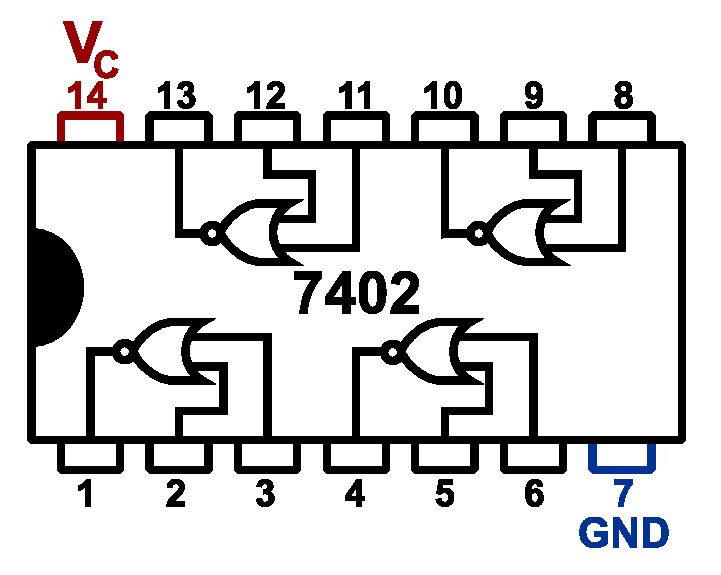
\includegraphics[scale=0.45]{grafiki/TTL_NOR_7402.eps}
            \caption{Schemat układu 7402 z bramkami NOR -- opis wejść/wyjść,
            \\Źródło: Opracowanie własne}
        \end{figure}

        Z pomocą impulsatorów zostały dokonane testy każdej z bramek (1,2,3), (4,5,6), (8,9,10) oraz (11,12,13).

        \begin{figure}[!ht]
          \centering
          \includegraphics[scale=0.09]{grafiki/NOR_1_2_3_test.png}
          \caption{Poprawna reakcja Bramki (1,2,3) układu 7402 na dwie bitowe jedynki (spadek napięcia),
          \\Źródło: Opracowanie własne}
        \end{figure}
        Żadna z bramek nie wykazała błędnego działania. Na powyższym rysunku jesteśmy wstanie zauważyć poprawną rekację jednej z nich. Wyjścia $Q$ impulsatorów zostały wpięte na wejścia $2$ oraz $3$ układu a wyjście $1$ jest obrazowane na ekranie oscyloskopu. Jak jesteśmy wstanie dostrzec na ekranie oscyloskopu, gdy oba przyciski nie były wciśnięte, sygnał pozywał ok. $4V$ co odbierane jest jako stan wysoki.

      \subsubsection{EXOR(7486)}
        Żeby zbadać wejścia oraz wyjścia układu na początku został sporządzony schemat działania układu. Użyta została dokumentacja układu dostępna w Internecie. Przedstawiony poniżej schemat został zmodyfikowany tak, jak wejścia na płytce UC-2 aby uprościć opis zadań.

        \begin{figure}[!ht]
            \centering
            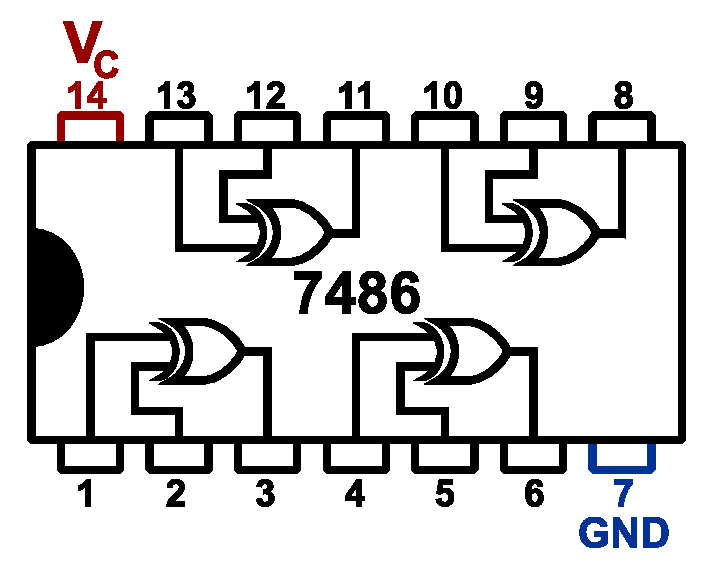
\includegraphics[scale=0.45]{grafiki/TTL_EXOR_7486.eps}
            \caption{Schemat układu 7486 z bramkami EXOR -- opis wejść/wyjść,
            \\Źródło: Opracowanie własne}
        \end{figure}

        Z pomocą impulsatorów zostały dokonane testy każdej z bramek (1,2,3), (4,5,6), (8,9,10) oraz (11,12,13).

        \begin{figure}[!ht]
          \centering
          \includegraphics[scale=0.09]{grafiki/EXOR_1_2_3_test.png}
          \caption{Poprawna reakcja Bramki (1,2,3) układu 7486 na jedną bitową jedynkę i jedno zero (wzrost napięcia),
          \\Źródło: Opracowanie własne}
        \end{figure}
        Żadna z bramek nie wykazała błędnego działania. Na powyższym rysunku jesteśmy wstanie zauważyć poprawną rekację jednej z nich. Wyjścia $Q$ impulsatorów zostały wpięte na wejścia $1$ oraz $2$ układu a wyjście $3$ jest obrazowane na ekranie oscyloskopu. Jak jesteśmy wstanie dostrzec na ekranie oscyloskopu, wciśnięcie jednego przycisku, wywołuje pożądany wrost napięcia.

    \subsection{Ćwiczenie 4.3}
        Zadanie numer 3 polegało na zrealizowaniu operacji negacji, iloczynu oraz sumy przy użyciu tyko jednego typu bramki. Użyte do tego zostały schematy na rysunku(\ref{fig1:Operacje}).

        \subsubsection{Realizacja przy użyciu bramek NAND}

        \begin{figure}[!ht]
          \begin{minipage}{.33\textwidth}
            \centering
            \includegraphics[scale=0.09]{grafiki/Negacja_NAND.png}
            \caption{Operacji negacji zrealizowana przy użyciu bramki NAND,
            \\Źródło: Opracowanie własne}
          \end{minipage}
          \begin{minipage}{.33\textwidth}
            \centering
            \includegraphics[scale=0.08]{grafiki/Iloczyn_NAND.png}
            \caption{Operacji iloczynu zrealizowana przy użyciu bramki NAND,
            \\Źródło: Opracowanie własne}
          \end{minipage}
          \begin{minipage}{.33\textwidth}
            \centering
            \includegraphics[scale=0.09]{grafiki/Suma_NAND.png}
            \caption{Operacji sumy zrealizowana przy użyciu bramki NAND,
            \\Źródło: Opracowanie własne}
          \end{minipage}
        \end{figure}
        \textbf{Negacja} \\
        W tej implementacji została użyta jedna bramka z wejściami $1$ oraz $2$ na które podawany jest ten sam sygnał. Wyjście posiada numer $3$.

        \textbf{Iloczyn} \\
        Do stworzenia układu wykonującego iloczyn potrzebne były dwie bramki NAND. Skorzystałem z bramek (1,2,3) oraz (4,5,6). Układ przyjmował sygnał na wejścia  $1$ oraz $2$. Wynik operacji natomiast był dostępny na wyjściu numer $6$.

        Obie bramki zostały połączone poprzez wpięcie wyjścia $3$ na wejścia $4$ oraz $5$.

        \textbf{Suma} \\
        Funkcja logiczna sumy potrzebowała już 3 wykorzystanych bramek (1,2,3), (4,5,6) oraz (13,12,11). Pierwsza i ostatnia bramka przyjmowały ten sam sygnał na oba wejścia a wyjścia $3$ oraz $11$ zostały podłączone do drugiej bramki. Wynik uzyskujemy na wyjściu numer $6$.
        \pagebreak

        \subsubsection{Realizacja przy użyciu bramek NOR}

        \begin{figure}[!ht]
          \begin{minipage}{.33\textwidth}
            \centering
            \includegraphics[scale=0.07]{grafiki/Negacja_NOR.png}
            \caption{Operacji negacji zrealizowana przy użyciu bramki NOR,
            \\Źródło: Opracowanie własne}
          \end{minipage}
          \begin{minipage}{.33\textwidth}
            \centering
            \includegraphics[scale=0.07]{grafiki/Iloczyn_NOR.png}
            \caption{Operacji iloczynu zrealizowana przy użyciu bramki NOR,
            \\Źródło: Opracowanie własne}
          \end{minipage}
          \begin{minipage}{.33\textwidth}
            \centering
            \includegraphics[scale=0.07]{grafiki/Suma_NOR.png}
            \caption{Operacji sumy zrealizowana przy użyciu bramki NOR,
            \\Źródło: Opracowanie własne}
          \end{minipage}
        \end{figure}
        \textbf{Negacja} \\
        W tej implementacji została użyta jedna bramka z wejściami $2$ oraz $3$ na które podawany jest ten sam sygnał. Wyjście posiada numer $1$.

        \textbf{Iloczyn} \\
        Funkcja logiczna iloczynu potrzebowała już 3 wykorzystanych bramek (1,2,3), (4,5,6) oraz (13,12,11). Pierwsza i ostatnia bramka przyjmowały ten sam sygnał na oba wejścia a wyjścia $1$ oraz $13$ zostały podłączone do drugiej bramki. Wynik uzyskujemy na wyjściu numer $4$.

        \textbf{Suma} \\
        Do stworzenia układu wykonującego sumę potrzebne były dwie bramki NOR. Skorzystałem z bramek (1,2,3) oraz (4,5,6). Układ przyjmował sygnał na wejścia $2$ oraz $3$. Wynik operacji natomiast był dostępny na wyjściu numer $4$.

        Obie bramki zostały połączone poprzez wpięcie wyjścia $1$ na wejścia $5$ oraz $6$.

    \subsection{Ćwiczenie 4.4}
      Zadanie czwarte dotyczyło wyznaczenia średniego czas propagacji impulsu przez bramkę mierząc okres drgań generatora zbudowanego z trzech bramek. Do budowy generatora miały być użyte bramki 7400 oraz 74S00.

        \begin{figure}[!ht]
          \centering
          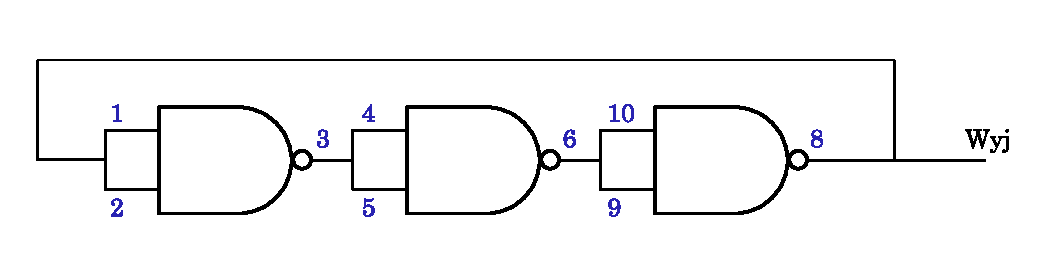
\includegraphics[scale=0.55]{grafiki/3_NAND.eps}
          \caption{Schemat generatora który miał zostać zbudowany w tym zadaniu (przy użyciu bramek NAND),
          \\Źródło: Opracowanie własne}
        \end{figure}
      Powyższy schemat został dodatkowo wzbogacony o numery wejść/wyjść jakie zostały użyte przy budowie układu na płytce UC-2.
      Sygnał uzyskany z bramek został wpuszczony na oscylator przez kanał 1 który posiadał oporność $1M\Omega$.

      \pagebreak
    \subsubsection{7400}
      Jak jesteśmy wstanie zaobserwować, okres drgań dla układu 4700 wynosi ok. $66,4ns$. 
    \begin{figure}[!ht]
      \begin{minipage}{.5\textwidth}
        \centering
        \includegraphics[scale=0.07]{grafiki/3_NAND_zdj.png}
        \caption{implementacja generatora zbudowana przy użyciu bramek NAND 4700,
        \\Źródło: Opracowanie własne}
      \end{minipage}
      \begin{minipage}{.5\textwidth}
      \centering
      \includegraphics[scale=0.35]{grafiki/7400_pomiar.png}
      \caption{Pomiar okresu drgań generatora zbudowanego z bramek NAND 4700,
      \\Źródło: Opracowanie własne}
      \end{minipage}

    \end{figure}

    \subsubsection{74S00}
      W tym przypadku natomiast okres drgań jest miejszy, wynoszący ok. jedynie $20,6ns$. Różnicę zauważyć idzie również w amplitudzie która zamiast $5V$ wskazuje tylko okolice $2V$.
      \begin{figure}[!ht]
        \begin{minipage}{.5\textwidth}
          \centering
          \includegraphics[scale=0.07]{grafiki/3_NAND_zdj_2.png}
          \caption{implementacja generatora zbudowana przy użyciu bramek NAND 47S00,
          \\Źródło: Opracowanie własne}
        \end{minipage}
        \begin{minipage}{.5\textwidth}
          \centering
          \includegraphics[scale=0.35]{grafiki/74S00_pomiar.png}
          \caption{Pomiar okresu drgań generatora zbudowanego z bramek NAND 47S00,
          \\Źródło: Opracowanie własne}
        \end{minipage}
      \end{figure}

    \subsection{Ćwiczenie 4.5}
      Zadanie to było robione na końcu zajęć oraz polegało na zbudowaniu funkcji logicznej dla jednego wybranego segmentu (a, b, c, d, e, f, g) wskaźnika 7-segmentowego, którego zadaniem będzie wyświetlanie liczb w systemie ósemkowym. 
      \pagebreak
      \begin{figure}[!ht]
        \begin{minipage}{.5\textwidth}
          \centering
          \includegraphics[scale=0.55]{grafiki/wyswietlacz.jpg}
          \caption{Zdjęcie poglądowe wyświetlacza z podpisanymi segmentami,
          \\Źródło: \href{https://spe.if.uj.edu.pl/literatura}{Strona wykładów}}
            \end{minipage}
          \begin{minipage}{.5\textwidth}
        \centering
        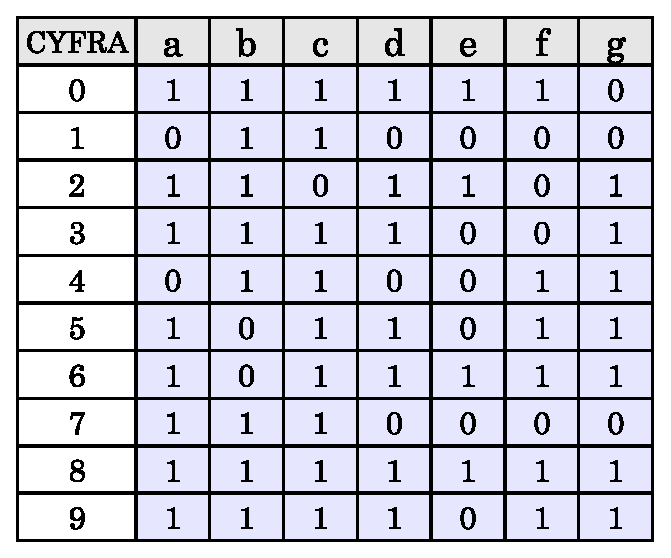
\includegraphics[scale=0.65]{grafiki/wyswietlacz_segmenty_tabela.eps}
        \caption{Tabela przedstawiająca stany dla każdego możliwego segmentu wyświetlacza,
        \\Źródło: \href{https://spe.if.uj.edu.pl/literatura}{Strona wykładów}}
          \end{minipage}
      \end{figure}

      Do zbudowania wybrany został segment $a$. Każda z liczb została rozpisana binarnie na bity w celu stworzenia mapy Karnaugh.

      \begin{figure}[!ht]
        \begin{minipage}{.5\textwidth}
            \centering
            \begin{tabular}{|c|c|c|}
            \hline
            \textbf{Binarnie (ABCD)} & \textbf{Cyfra} & \textbf{Segment A} \\
            \hline
            0000 & 0 & 1 \\
            \hline
            0001 & 1 & 0 \\
            \hline
            0010 & 2 & 1 \\
            \hline
            0011 & 3 & 1 \\
            \hline
            0100 & 4 & 0 \\
            \hline
            0101 & 5 & 1 \\
            \hline
            0110 & 6 & 1 \\
            \hline
            0111 & 7 & 1 \\
            \hline
            1000 & 8 & 1 \\
            \hline
            1001 & 9 & 1 \\
            \hline
            \end{tabular}
            \caption{Reakacja segmentu $A$ dla poszczególnych liczb wraz z ich binarnym zapisem,
            \\Źródło: Opracowanie własne}
        \end{minipage}
        \begin{minipage}{.5\textwidth}
          \centering
          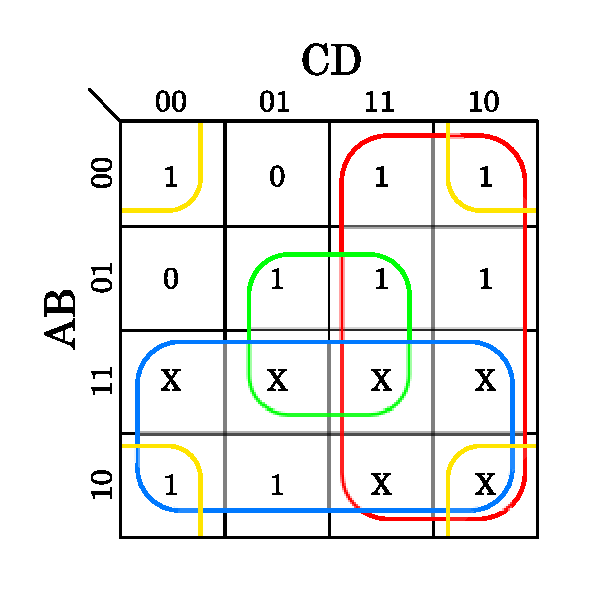
\includegraphics[scale=0.65]{grafiki/K_map_segment_a.eps}
          \caption{Mapa Karnaugh stworzona w celu minimalizacji funkcji logicznej,
          \\Źródło: Opracowanie własne}
        \end{minipage}
      \end{figure}

      Funkcja po zminimalizowaniu mapą Karnaugh prezentuje się nastepująco: \\
      \begin{equation}
        \textcolor{red}{C} + \textcolor{blue}{A} + \textcolor{green}{BD} + \textcolor{yellow}{\overline{B}\ \overline{D}}
      \end{equation}

      Znaki $X$ oznaczają dowolne pola, czyli takie których stan nas nie interesuje. Pozwala to na większą minimalizacje w sytuacji gdy ustawimy je wszystkie na wartość $1$.

      \begin{figure}[!ht]
        \centering
        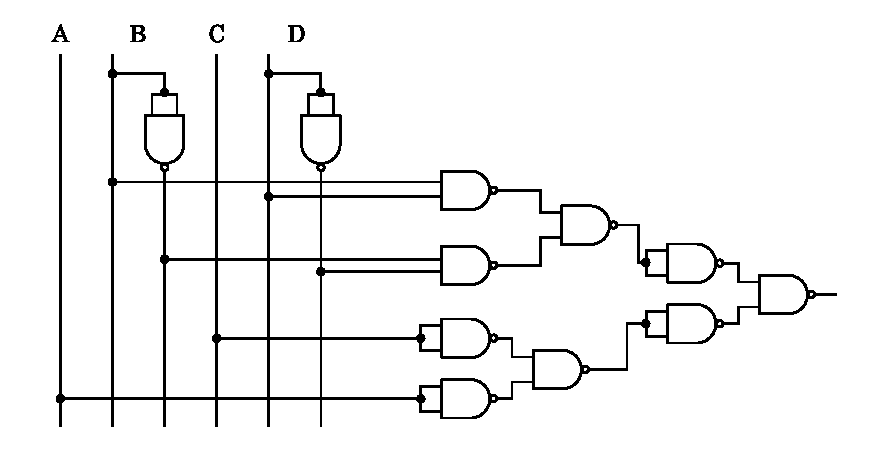
\includegraphics[scale=0.65]{grafiki/schemat_segment_a.eps}
        \caption{Schemat segmentu $a$ wykonanu przy użyciu tylko bramek NAND,
        \\Źródło: Opracowanie własne}
      \end{figure}
      \pagebreak

    \subsection{Ćwiczenie 4.6}
      Ostatnim zadaniem było zaprojektowanie układu działającego jak przerzutnik asynchroniczny RS. Na widoczym poniżej schemacie zostały dopisane numery wejść/wyjść z których skorzystano przy jego budowie.
      
      \begin{figure}[!ht]
        \begin{minipage}{.5\textwidth}
          \centering
          \includegraphics[scale=0.07]{grafiki/RS_przerzutnik_zdj.png}
          \caption{Poprawnie zmontowany układ RS z wykorzystaniem bramek NAND,
          \\Źródło: Opracowanie własne}
            \end{minipage}
          \begin{minipage}{.5\textwidth}
        \centering
        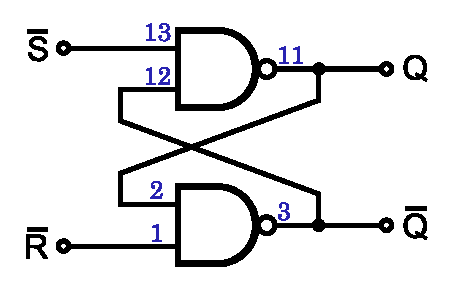
\includegraphics[scale=0.65]{grafiki/SR_NAND_schemat_wej_wyj.eps}
        \caption{Schemat przerzutnika RS zbudowanego z bramek NAND z podpisanymi numerami wejść/ wyjść,
        \\Źródło: Opracowanie własne}
          \end{minipage}
      \end{figure}

      Sposób działania układu został przeze mnie zarejestrowany cyfrowo w formie filmu.\href{https://youtu.be/9eNzdQyRCHI}{[Link do nagrania]}. Na jego podstawie została stworzona tablica stanów układu.

      Górny impulsator na płytce służył jako wejście $RESET$ a dolny jako $SET$.
      Warto zauważyć, że przerzutnik, nawet gdy wejścia pozostają odpięte od źródła zasilania, ``pamięta'' swój stan.
      \begin{table}[h]
        \centering
        \begin{tabular}{|c|c|c|c|}
        \hline
        \footnotesize $\mathbf{\overline{S}}$ & \footnotesize $\mathbf{\overline{R}}$ & \footnotesize $\mathbf{Q_n}$ & \footnotesize $\mathbf{\overline{Q_n}}$ \\
        \hline
        0 & 0 & stan zabroniony & stan zabroniony \\
        \hline
        0 & 1 & 1 & 0 \\
        \hline
        1 & 0 & 0 & 1 \\
        \hline
        1 & 1 & stan pamiętania & stan pamiętania \\
        \hline
        \end{tabular}
        \caption{Tablica prawdy dla przerzutnika RS zbudowanego nan NAND'ach}
      \end{table}

    

  \section{Omówienie wyników}
    \subsection{Ćwiczenie 4.1}
      Każda z funkcji płytki działa poprawnie. Nie zostały napotkane żadne anomalie podczas przeprowadzania pomiarów kontrolnych.
    \subsection{Ćwiczenie 4.2}
      We wszyskich 3 układach sprawdzone zostały każde z wejść oraz wyjść. Każde z nich dawało oczekiwany wynik względem odpowiadających im bramek. Odczyt z oscyloskopu we każdym z przypadków utrzymywał się w granicach przewidywanego napięcia wyjściowego --- przyjmował wartości ok. $4V$ w stanie wysokim.
    \subsection{Ćwiczenie 4.3}
      Dla każdego ze zbudowanych układów logicznych proces przebiegł pomyślnie. Układy odpowiadały według tablic prawdy im odpowiadających (\ref{fig2:brameczki}). Potwierdza to fakt, że przy pomocy tylko bramek NAND bądź NOR można zbudować każda funkcję logiczną.
    \subsection{Ćwiczenie 4.4}
      Budowę zdanego układu udało wykonać zgodnie z planem. Udało się uzyskać pożądany efekt drgań. Niestety odczyt wykonany z użyciem oscyloskopu nie został przeprowadzony równie uważnie. Samo wyświetlenie napięcia wyjściowego zostało jak najbardziej wykonane, łącznie z prostym pomiarem okresu drgań. Jednak z niewiadomych przyczyn zapisany został tylko screenshot z napięciem wyjściowym, bez $U_{WE}$. Uniemożliwiło to w poźniejszym procesie obliczenie wymaganego czasu propagacji impulsu.

      To co możemy wywnioskować z uzyskanych okresów to to, że wersja $47S00$ jest szybsza od zwykłego układu $4700$. Pokrywa się to z informacjami dostępnymi w sieci które wprost mówią, że jest to seria pochodnych, wykonywana w technologiach S, czyli o podwyższonej szybkości.
    \subsection{Ćwiczenie 4.5}
      Z racji wykonywania tego zadania na samym końcu zajęć, zostało ono wpierw wykonane z błędem. Wykrycie złej funkcjonalności odkryto dopiero na etapie testowania zbudowanego układu. Błąd polegał na zinterpretowaniu pól \textit{X} jako zer zamiast jedynek. Wybranie jedynek pozwoliło na stworzenie układu działającego według zadanej tablicy prawdy, jednak zostało dopiero dokonane na etapie pracy nad tym sprawozdaniem. Z tego też powodu zadanie nie posiada zdjęcia zbudowanego układu --- źle zbudowany został umieszczony w sekcji \textit{\textbf{Notatki z zajęć}}.

    \subsection{Ćwiczenie 4.6}
      Ostatnie zadanie przebiegło bez większych problemów, układ został zmontowany zmontowany pomyślnie. Ważnym aspektem tego układu jest faktyczne ``pamiętanie'' stanu, nawet podczas odpięcia wejść. Najlepiej obrazuje to nagranie wideo stworzone podczas zajęć.
  \section{Podsumowanie}
    Podsumowując, serie eksperymentów przyniosły różnorodne wnioski i doświadczenia. Zadania coraz bardziej wywierają nacisk na myślenie zamiast na wykonywaniu zadań bez zastanowienia. Wypracowuje to w studentach umiejętności potrzebne do samodzielnej pracy. Większość z ćwiczeń przebiegła pomyślnie, kilka zostały dotknięte czynnikiem ludzkim który nie zawsze jest perfekcyjny. Ważne jest, żeby brać pod uwagę zarówno sukcesy, jak i trudności, ponieważ oba mogą prowadzić do cennych wniosków i lepszych umiejętności w przyszłych projektach.
  \section{Notatki z zajęć}

  \begin{figure}[!ht]
    \begin{minipage}{.5\textwidth}
      \centering
      \includegraphics[scale=0.07]{grafiki/notatki1.jpg}
      \caption{Notatki sporządzone podczas sprawdzania bramek,
      \\Źródło: Opracowanie własne}
    \end{minipage}
    \begin{minipage}{.5\textwidth}
      \centering
      \includegraphics[scale=0.08]{grafiki/notatki2.jpg}
      \caption{Notatki wykonane podczas robienia zadań 4 oraz 6,
      \\Źródło: Opracowanie własne}
    \end{minipage}
  \end{figure}

  \begin{figure}[!ht]
    \begin{minipage}{.5\textwidth}
      \centering
      \includegraphics[scale=0.06]{grafiki/notatki3.jpg}
      \caption{tablica prawdy do segmentu $a$ z zadania 5,
      \\Źródło: Opracowanie własne}
    \end{minipage}
    \begin{minipage}{.5\textwidth}
      \centering
      \includegraphics[scale=0.08]{grafiki/notatki4.jpg}
      \caption{ Poprawny schemat z bramek NAND do zadania 5, wykonany w czasie późniejszym,
      \\Źródło: Opracowanie własne}
    \end{minipage}
  \end{figure}


  \begin{figure}[!ht]
    \begin{minipage}{.5\textwidth}
      \centering
      \includegraphics[scale=0.07]{grafiki/notatki5.jpg}
      \caption{Błędne obliczenia dotyczące zadania 5,
      \\Źródło: Opracowanie własne}
    \end{minipage}
    \begin{minipage}{.5\textwidth}
      \centering
      \includegraphics[scale=0.06]{grafiki/bledny_uklad_zad_5.png}
      \caption{Błędne zbudowany układ z zadania 5,
      \\Źródło: Opracowanie własne}
    \end{minipage}
  \end{figure}


\end{document}